All code is found at https://github.com/Oscarlsson/RL-competition

When testing our agent on very different environments, from simple board games to context bandit problems. We observe that even very general approaches to improving performance against a large class of environments, might deteriorate the performance against other environments. We attempted ike environments where the state is altered gradually and good actions are good over a range of similar states

Running the agent with varying step sizes $\alpha$ we observed bad results on all values but $\alpha=1$.


Sweep $\lambda$
\begin{figure}[h]
    \centering
    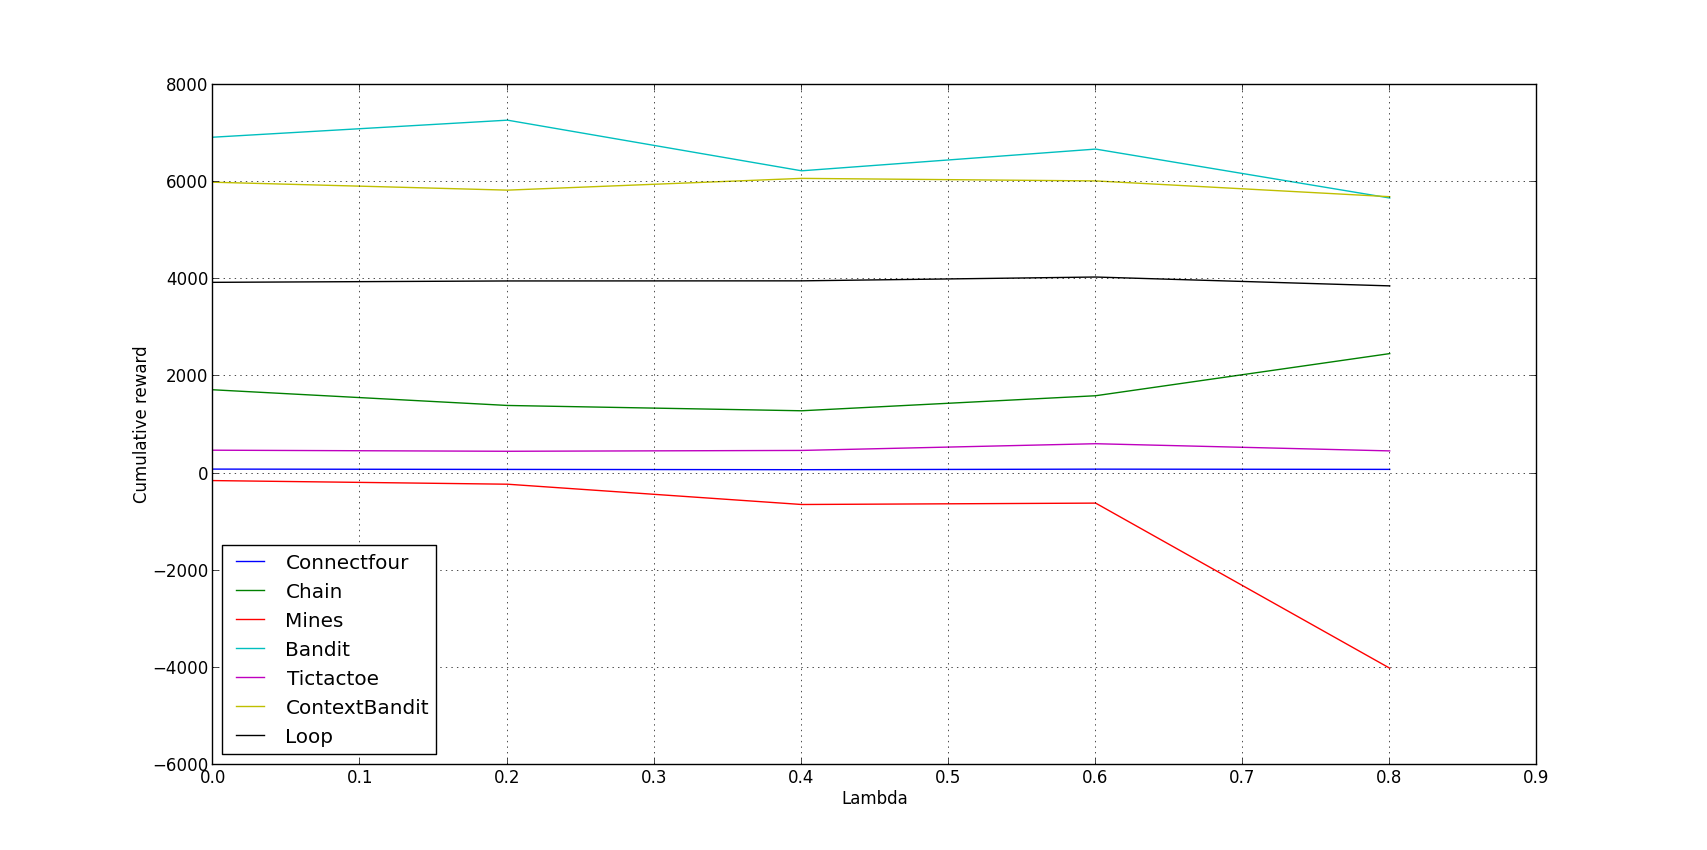
\includegraphics[width=0.5\textwidth]{../data/lambdasweepplot.png}
    \caption{Awesome Image}
    \label{fig:awesome_image}
\end{figure}


Figure~\ref{fig:cumreward} shows how the agents average performance over 50 runs in a 100 episode experiment against all environments with parameters set to $\lambda = 0.2$ and $\alpha = 1$

\begin{figure}[h!]
    \centering
    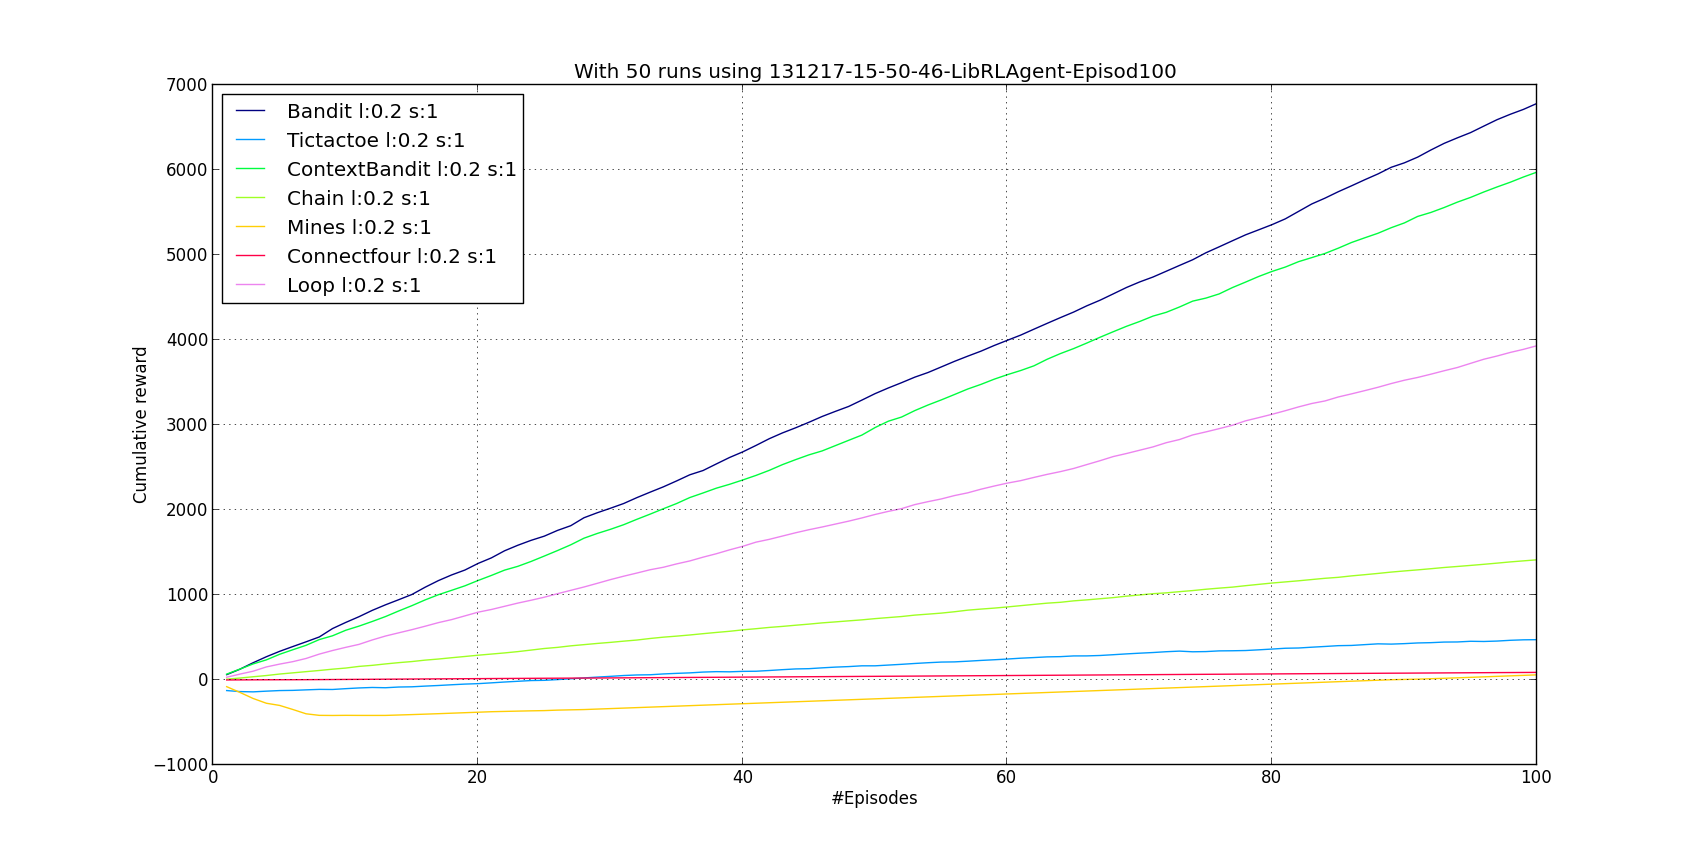
\includegraphics[width=0.5\textwidth]{../data/100episodes_50runs.png}
    \caption{Agents cumulative reward averaged over 50 runs}
    \label{fig:cumreward}
\end{figure}

The yellow line indicates the performance on the mines environment and the learning phase of the agent is clear after around 10 episodes. Connect four, red in Fig~\ref{fig:cumreward}, has a much lower maximum reward than the other environments hence it is closer to zero but still increasing.
